%%%%%%%%%%%%%%%%%%%%%%%%%%%%%%%%%%%%%%%%%%%%%%%%%%%%%%%%%%%%%%%%%%%%%%%%%%%%%%%%%
%                                                                               %
%                        ELEN4009: Software Engineering                         %
%                                                                               %
%          The Online Postgraduate Application Approval System for EIE          %
%                     Document Adapted from IEEE Template                       %
%                                                                               %
%                         Lecturer: Professor E. Otoo                           %
%                                                                               %
%      Front-End: Nomakhosi Ndebele (671480) and Timothy Rokebrand (458960)     %
%           Back-End: Julio Baeta (710066) and Ryan Robinson (453764)           %
%                                                                               %
%                       University of the Witwatersrand                         %
%                                                                               %
%              School of Electrical and Information Engineering                 %
%                                                                               %
%%%%%%%%%%%%%%%%%%%%%%%%%%%%%%%%%%%%%%%%%%%%%%%%%%%%%%%%%%%%%%%%%%%%%%%%%%%%%%%%%

\documentclass[journal]{IEEEtran}

\usepackage{fancyhdr}
\usepackage{graphicx}

\pagestyle{fancy}

\renewcommand{\headrulewidth}{0pt}

\begin{document}

\title{ELEN4009 - Software Engineering\\ The Online Postgraduate Application\\ Approval System for EIE}

\author{\vspace{2mm} \small School of Electrical \& Information Engineering, University of the Witwatersrand, Private Bag 3, 2050, Johannesburg, South Africa \vspace{1mm} \\ \normalsize Front-End: Nomakhosi Ndebele (671480) and Timothy Rokebrand (458960) \\ Back-End: Julio Baeta (710066) and Ryan Robinson (453764)
}

% The paper headers
\markboth{}{}

\maketitle

%%%%%%%%%%%%%%%%%%%%%%%%%%%%%%%%%%%%%%%%%%%%%%%%%%%%%%%%%%%%%%%%%%%%%%%%%%%%%%%%%

\thispagestyle{fancy}

\begin{abstract}

This report serves as an overview of the online postgraduate application system that was designed to be used by the School of Electrical and Information Engineering within the University of the Witwatersrand. The basic system consisted of both front- and back-end modules, both of which are discussed at length herein. The design presented within this report is a very high-level architecture of a system that could be used as a final product. Consequently, there is a significant amount of room for additional implementations to be incorporated into the system, as well as improvements to the current implemented design. Although high-level, the design was deemed to be a success by virtue of the fact that the criteria set out for it at the beginning of the project were met, with only a few design compromises having to be made.

\end{abstract}

\IEEEpeerreviewmaketitle

%%%%%%%%%%%%%%%%%%%%%%%%%%%%%%%%%%%%%%%%%%%%%%%%%%%%%%%%%%%%%%%%%%%%%%%%%%%%%%%%%

\section{Introduction}

The University of the Witwatersrand (Wits) is one of the leading universities in South Africa \cite{topuniversity}. For the 2016 academic year, Wits received in excess of 70 000 first-year applications across all faculties \cite{witsapplicants}. This statistic justifies the fact that the application process to the university needs to be made as efficient and reliable as possible. This project focusses specifically on the postgraduate application process to the School of Electrical and Information Engineering within Wits. The implementation of a completely electronic application system would not only reduce the amount of paperwork required to be handled by the relevant staff members within the school, but also provide a platform on which other faculties could base similar types of systems for their specific application processes. 

%%%%%%%%%%%%%%%%%%%%%%%%%%%%%%%%%%%%%%%%%%%%%%%%%%%%%%%%%%%%%%%%%%%%%%%%%%%%%%%%%

\section{Problem Definition}

The postgraduate application process to the School of Electrical and Information Engineering is one that has always been marred by a significant amount of paperwork that is required to be printed for each applying student. This situation is problematic not only in terms of administrative duties for those handling the paperwork, but is also not an environmentally-friendly process, due to all the paper that is used in printing each applicant's documentation.

\hfill \break One proposed solution to this problem is to make each applicant's information and relevant documentation readily available to the school through an online system. This will enable quick access to each student's information, reduce the amount of paper used and enable everyone involved in the decision-making process for a particular applicant to be able to communicate their perspectives and decisions with one another through the system.

%%%%%%%%%%%%%%%%%%%%%%%%%%%%%%%%%%%%%%%%%%%%%%%%%%%%%%%%%%%%%%%%%%%%%%%%%%%%%%%%%

\section{System Objectives}

In order for the project to be completed successfully, a set of success criteria needed to be clearly set out before any form of work could be carried out. It is important to note that the scope of this project extends only to a very high-level design. It was not required for a fully functional system to be designed and implemented. As such, a very simple prototype of the final system that may be created for the school by an outsourced software company was produced.

\hfill \break The success criteria of a fully functional final product are as follows:

\begin{enumerate}
	\item The system must be capable of receiving and storing all student information obtained from the Student Information Management Systems (SIMS) department at the university. The system must also be capable of sending a decision regarding their application back to SIMS once the application process is complete.
	\item All student credentials must be stored within a database that can be accessed by the interface of the system. These credentials include the applicant's name, person number, contact number, potential supervisor name, university where the applicant completed their undergraduate degree, the program in which they are interested in as well as the status of their application.
	\item All of the student's required documentation must be stored within a text database that can also be accessed by the interface of the system. These documents include academic transcripts, certificates of qualification, curriculum vitaes (CVs) and identity documents. Search functionality should be incorporated within this database, such that specific information pertaining to a particular student can be located quickly.
	\item The user interface must be simple to learn, understand, and use as well as being as graphically pleasing as possible.
	\item All information stored within the system's databases must be secure and inaccessible to anyone that is not involved within the application process, as some of this information is sensitive and cannot afford to be lost to anyone outside of the university.
	\item The information that is accessible to each user is determined by their level of involvement within the application process. For example, a supervisor in the field of High Voltage Engineering will not have access to information pertaining to applicants who are interested in Telecommunications Engineering.
\end{enumerate}

\hfill \break Due to the primary objective of the project being to implement a simple prototype that simply displays the very basic functionality of such a system, only select aspects of these success criteria were implemented within this scope. These include:

\begin{enumerate}
	\item A very rudimental login page that can be surpassed by any input being placed into the `Person Number' and `Password' fields.
	\item A basic information page that displays a list of all applicants, their potential supervisors and the program in which they are interested.
	\item A more information comprehensive page (for each student) that features a listing of all their information and relevant documentation.
	\item A database for storing each student's information, as well as a database to store each student's required documentation.
\end{enumerate}

%%%%%%%%%%%%%%%%%%%%%%%%%%%%%%%%%%%%%%%%%%%%%%%%%%%%%%%%%%%%%%%%%%%%%%%%%%%%%%%%%

\section{System Architecture}

The architecture of the system will be two-tiered. The reason for this is that there is a very limited amount of data processing taking place within the system. The only data processing that will occur is database querying (searching and retrieval of information), application status toggling and the addition of supervisor comments.

%%%%%%%%%%%%%%%%%%%%%%%%%%%%%%%%%%%%%%%%%%%%%%%%%%%%%%%%%%%%%%%%%%%%%%%%%%%%%%%%%

\section{Assumptions}

To ensure that the system produced performed as expected and did not go out of the required scope, it is necessary for a number of assumptions to be worked under. These include:

\begin{enumerate}
	\item All information and documentation for each student that is required to be obtained from SIMS has already been retrieved.
	\item All information and documentation received is in the correct format and will not need to be converted.
	\item All information relating to each student is correct and will not require any form of rectification.
	\item The system is hosted on a server within the School of Electrical and Information Engineering.
\end{enumerate}

%%%%%%%%%%%%%%%%%%%%%%%%%%%%%%%%%%%%%%%%%%%%%%%%%%%%%%%%%%%%%%%%%%%%%%%%%%%%%%%%%

\section{Software Development Life Cycle - Scrum}

The greatest obstacle faced by the software development team was the very limited amount of time in which the project could be completed. As such, it was essential that the choice of software development methodology adopted allowed for the project to be completed thoroughly and in the shortest amount of time possible. For this reason, the Scrum methodology was utilised. Scrum requires a number of roles to be defined as follows.

\subsection{Product Owner}

The owner of the product, or rather the customer for who the system is being produced is the School of Electrical and Information Engineering at Wits.

\subsection{System Users}

The primary user of the system would be the postgraduate officer within the school, Ms Mumtaz Adam. The postgraduate course coordinator, Mr Ivan Hofsajer, would also be making extensive use of the system. The other users of the system would be the supervisors for the various fields of interest being offered to applicants.

\subsection{Other Stakeholders}

Only two other departments at Wits would have stakes within this project, namely SIMS (as mentioned in section III above), which manages all information pertaining to students, as well as the Student Enrolment Centre (SEnC), which handles all applications to the university in some form or another.

\hfill \break In order for the Scrum methodology to be correctly carried out, it was also necessary for certain roles within the software development team itself to be established. This involved deciding on which developers would work on the front-end aspect of the system, which developers would work on the back-end aspect and who would lead the project in the form of a Scrum Master \cite{ProfOtoo}.

\subsection{Front-End Module Developers}

The responsibility of designing the user interface and how the various web pages within the system would link up to one another was assigned to Nomakhosi Ndebele and Timothy Rokebrand.

\subsection{Back-End Module Developers}

The duties of designing and implementing the two databases to contain student information as well as each student's relevant documentation was given to Julio Baeta and Ryan Robinson.

\subsection{Scrum Master}

The role of Scrum Master, an individual who would consult with the course lecturer on a regular basis and ensure that the project was running efficiently and on schedule, was assigned to one of the software development team. This was as a result of there being no other individual available to the team (that wasn't one of the software developers themselves) to fulfil this role. As such, this role was assigned to Ryan Robinson.

\hfill \break The Scrum methodology implies that work would be divided into a number of segments (called sprints) and that regular sprint planning meetings would need to be held.

\subsection{Sprints}

Sprint planning meetings were held once a week, due to the project being very short in nature and needing to be completed within the shortest time frame possible. At each meeting, the previous sprint's successful and weak aspects were identified and discussed. This then allowed for subsequent sprints to not suffer from the same problems that previous sprints had, thus maximising productivity levels.

\hfill \break It is worth noting that within industry, usually the product owner is present at all Scrum meetings in order to ensure that the final system produced meets their requirements. However, due to the implementation only being a very high-level one, this aspect of Scrum could not be fulfilled. Instead, the course lecturer was consulted on a regular basis to ensure that the intended requirements were met as closely as possible.

\hfill \break Another aspect of Scrum that could not be fulfilled was that of daily Scrum meetings. These are usually held to ensure that all members of the software development team are well coordinated and understand exactly what is required of them before the beginning of the upcoming day's activities. Due to the members of the software development team having a variety of commitments, this aspect could not be satisfied within the scope of this project.

%%%%%%%%%%%%%%%%%%%%%%%%%%%%%%%%%%%%%%%%%%%%%%%%%%%%%%%%%%%%%%%%%%%%%%%%%%%%%%%%%

\section{User Hardware Requirements}

A very basic hardware setup is required for the computers that will be operating the online application system. Any computer that is capable of operating a web browser and which has an internet connection will be able to run the system.

%%%%%%%%%%%%%%%%%%%%%%%%%%%%%%%%%%%%%%%%%%%%%%%%%%%%%%%%%%%%%%%%%%%%%%%%%%%%%%%%%

\clearpage

%%%%%%%%%%%%%%%%%%%%%%%%%%%%%%%%%%%%%%%%%%%%%%%%%%%%%%%%%%%%%%%%%%%%%%%%%%%%%%%%%

\section{Front-End Module}
Basically front-end development is the portion that the clients deal with in website development. This is achieved by making use of the CSS and HTML software which will be explained in detail in this section. The development process of the front-end will be discussed in this section.


%%%%%%%%%%%%%%%%%%%%%%%%%%%%%%%%%%%%%%%%%%%%%%%%%%%%%%%%%%%%%%%%%%%%%%%%%%%%%%%%%

\subsection{Requirement Specification}
This section reviews the requirements by the product owner. The standard of the IEEE software-based systems will be followed. 
\hfill \break \subsubsection{Purpose}
The main purpose of this postgraduate application approval system project is to ensure that the application process proceeds in the smoothest possible fashion for students as well as being user-friendly for the administrative staff who will be making use of the system during the course of a student's application.
\hfill \break \subsubsection{Target Audience}
There are three individuals (Administrative staff at the University of the Witwatersrand) meant to use this this product, the course coordinator, the particular Supervisor for the topic being applied for and the Post Graduate Officer.
\hfill \break \subsubsection{Scope}
The primary function of the designed software product will be to inform the student (following their application) as to whether they have been accepted into the postgraduate program or if they have been rejected in the fastest possible time. The designed product is intended to be solely used by the administrative staff involved in the application decision process.
\hfill \break \subsubsection{Product Features}
The system is capable of displaying specific student information, such as contact details, place of residence address and person number. The system is also able to display relevant student documentation, such as CVs, academic transcripts as well as a copy of their degree certificate the system is designed in such a way that it is user friendly, it allows for ease of access.  The system allows for comments to be placed on final decision, furthermore the system offers input options when necessary during the course of the application, e.g. when a supervisor needs to submit his decision, there is a text box that allows for the Supervisor to put the decision. 
\hfill \break \subsubsection{Users of the Online Application System }
The postgraduate officer (currently Ms Mumtaz Adam within the School of Electrical and Information Engineering) is one of the users of the system. This user will have wide access across the various web pages, but will not be able to access the decision-making section of the system. Supervisors (current lecturers within the school) also play a role in the system. These users will have access to only relevant student information of applicants who are interested in their field of specialty. The supervisors will have the authority to make decisions and comments, but will not be able to make any form of final decision. The postgraduate course coordinator (currently Professor Ivan Hofsajer) also has access to this system. This user will be able to view to all aspects of any applying student's information. This user will also be able to view and extend on the comments that have already been made by the supervisors, as well as submitting the final decision to the application process.

\hfill \break \subsubsection{Operating Environment of the System}
The environment in which the system will be run will be any form of web browser that is compatible with HTML5, HTTP/1.1 as well as CSS3. The browser will also need to support PHP, in order to form the link between the databases being used to store student information and the user interface. The system itself was programmed and tested in Linux. The hardware requirements of the system that will be running the online application system will be very basic, and most modern computers will be more than capable of running the system.
\hfill \break \subsubsection{User Documentation}
A basic user reference manual will be made available to anyone who intends to make use of the system.
\hfill \break \subsection{System Feature 1 – Preprogramed Responses}
When the Post graduate office wishes to provide a comment as to why an application is unable to be processed, a list of preprogrammed responses will appear in the form of a drop-down menu. This will provide an easier way for the postgraduate officer to respond to generic problems that may be experienced when a student does not provide the necessary documentation and information.
\hfill \break \subsubsection{System Feature 2 –System Segmentation}
Access is only granted to a member of the administrative staff when their input is required. This is a measure to ensure that time is not wasted on communication between the involved parties.
\hfill \break \subsubsection{System Feature 3 – User Accessibility}
The interface that will be viewed by the user will require very basic forms of input. It will thus be very simple to avoid any form of errors and miscommunications during the course of a student's application process.
\hfill \break \subsubsection{The Graphical User Interface (GUI)}
The front end interface of the system will be designed to be as user friendly as possible. This will create the most efficient and streamlined environment so that the software involved in the application process will not result in the user having a negative experience.
\hfill \break \subsubsection{Hardware and Software Interfaces }
There will be no form of hardware interface required to run the system, other than a standard desktop or laptop computer. In future, this hardware interface may be extended to include smart devices such as tablets or smartphones. Any form of internet browser may be used to operate this system. This includes Mozilla Firefox, Google Chrome, and Apple's Safari and Internet Explorer or Microsoft Edge can be used as well. 
\hfill \break \subsubsection{Software Quality Attributes}
The user interface will create a pleasant environment that all users should feel comfortable using. This will maximise productivity and reduce the amount of paper used in the postgraduate application process, thus making it an environmentally-friendly product.

%%%%%%%%%%%%%%%%%%%%%%%%%%%%%%%%%%%%%%%%%%%%%%%%%%%%%%%%%%%%%%%%%%%%%%%%%%%%%%%%%

\subsection{Design}
The front-end was created using various web-based languages namely, Hypertext Pre-processor (PHP), Hyper Text Mark-up Language 5 (HTML 5) and Cascading Style Sheets 3 (CSS 3). These languages worked in conjunction to provide the webpage with the necessary content and logic capabilities as well as styling. The following will give a detailed description of the roles each language played in the design of the system.
\hfill \break \subsubsection{HTML5} 
HTML is a language used to create pages for use on the World Wide Web. It defines the structure of the web page using a series of tags and assigning properties to certain sections of code \cite{html}. In terms of the project, HTML was used to provide the standard content to the pages such as titles and directions. The tables that would later be populated from information contained in the database were created using HTML code. It was also used to display any buttons and hyperlinks that were used to navigate elsewhere on the site.
\hfill \break \subsubsection{CSS3}
CSS is a style sheet language that is used to define how HTML outputs will be displayed to the end user \cite{css}.  In this project the style sheets were used to develop the layout, colour scheme, text and overall appearance of the pages throughout the website. One style template was developed from which all the other pages stylings were derived so as to ensure consistency in the appearance of the website as a whole. The aesthetics and layout of the page is important to help improve the usability of the page, as it ensures that everything is placed logically on the page to ensure the navigation between pages is simple and understood by all users.
\hfill \break \subsubsection{PHP}
PHP is a script language used widely on Linux-based web servers; it is used as a means to allow the web page to communicate with the database \cite{php}. In this project it was used to retrieve information from the MySQL database, in order to display the relevant student information when it was needed. It was used as HTML lacks the functionality to allow one to create variables and assign values to them, a process necessary to identify specific information in the database.
\hfill \break \subsubsection{Other files}
Files such as pictures that were used for aesthetics were stored in the server folder and retrieved via the HTML code where necessary.


%%%%%%%%%%%%%%%%%%%%%%%%%%%%%%%%%%%%%%%%%%%%%%%%%%%%%%%%%%%%%%%%%%%%%%%%%%%%%%%%%

\subsection{Implementation}
The implementation carried out was a basic, high-end version of what would be carried out in reality. The intention of the implementation carried out was to give an understanding of how a web page such as this could be designed and how interactions occur between the front-end and back-end. There were several elements that were not implemented which are spoken about in the critical analysis.

\hfill \break The base language for all the code produced for the front-end was HTML. Once the main structure was completed using HTML, the PHP and CSS code was added to complete the project. 

\hfill \break All the pages had the same basic design, only their contents changed. Using the `div' tag, each page was separated into different sections so as to make the editing of the page easier. All the information was contained in the body of the HTML code and all had the same main heading of “School of Electrical and Information Engineering”, this was then followed by tabs with links to the Home page and the Applicant List page; these were created using the list tags and hyperlinks in HTML, they were then edited using CSS to distinguish them from the rest of the page. The next section is what varied from page to page and that was the content of each page, but the formatting in terms of CSS remained consistent between the pages so as to ensure a sense of continuity for the user. 

\hfill \break Any page that required information from the database in order to complete the information contained on the page made use of PHP code amongst the HTML code. This was done in order to retrieve specific information from the database pertaining to the relevant student (discussed further in back-end section). In PHP sections the “echo” command had to be used when referring to HTML code so that it could output the relevant information to the user.


%%%%%%%%%%%%%%%%%%%%%%%%%%%%%%%%%%%%%%%%%%%%%%%%%%%%%%%%%%%%%%%%%%%%%%%%%%%%%%%%%

\subsection{Sprint Planning}
The following document is based on content found within the textbook ``Beginning Software Engineering" by Rod Stephens (pages 327 - 329) as well as lecture slides provided by Professor Otoo for the ELEN4009 course at the University of the Witwatersrand (2016). The Sprint planning meetings are meant to provide detailed development stages of the front-end. These were done at the same time as the back-end sprint planning meetings. In each of the meetings goals of the upcoming sprint and the plan to achieve the goal were discussed.  The details of the front-end weekly sprint planning meetings are provided.
\hfill \break \subsubsection{First Sprint Planning meeting (19 February)}
There were no objectives that needed to be completed, as it was the first formal sprint planning meeting. Previously only the project topic was chosen. The next sprint planning meeting required the knowledge of what software was to be used for the front-end portion. This was to be figured out before the next sprint planning meeting. In order to achieve this, research needed to be carried out into the provided software options given in the course brief.
\hfill \break \subsubsection{Second Sprint Planning meeting (26 February)}
In this sprint planning meeting all the required software for the front-end had been identified; PHP, HTML5 and CSS. There was little knowledge on how the software worked, so the goal for the next sprint meeting was to acquire the necessary knowledge regarding the software in order to progress with the front end development. 
\hfill \break \subsubsection{Third Sprint Planning meeting (4 March)}
This was aimed at discussing when a meeting could be held with the postgraduate officer in order to get clarity on what the School of Electrical and Information Engineering (product owner) expected from the development team. This was the goal to be achieved before the next sprint planning meeting.  Furthermore the information acquired from the postgraduate officer would help in the write up of the Systems Requirement Specifications (SRS) document.  In order to achieve this a meeting was arranged with the postgraduate officer.
\hfill \break \subsubsection{Forth Sprint Planning meeting (11 March)}
At this stage it was clear what was supposed to be done for the product owner, it was now possible to begin with the design and implementation of the front-end. The goal of the next sprint involved the design of web page layouts and how the navigation between them will occur. In order to achieve this goal the design was first done on paper to fully understand the flow of the layouts, tasks were divided into HTML and CSS.
\hfill \break \subsubsection{Fifth Sprint Planning meeting (18 March)}
The goal of the next Sprint was to start to implement the design (layouts of the pages) into HTML and CSS, for this to be successful each page layout was considered separately and all the individual pages were linked up.
\hfill \break \subsubsection{Sixth Sprint Planning meeting (29 March)}
The individual pages were available by this date and were ready to be integrated with the databases which the back-end team was working on. The integration process was achieved by explaining how the front end worked, which is the same way that the front end developers learned how the back-end operated. 
\hfill \break \subsubsection{Seventh Sprint Planning meeting (5 April)}
 The two modules were integrated by this date. The goal of the next sprint was to finalise the front and the back-end.  Furthermore the write up of all documentation needed to be finalised. \\

A summary of the planning process can be found in the form of a Gantt chart in figure 1, appendix A.

%%%%%%%%%%%%%%%%%%%%%%%%%%%%%%%%%%%%%%%%%%%%%%%%%%%%%%%%%%%%%%%%%%%%%%%%%%%%%%%%%

\subsection{Sprint Retrospective}
The approach to the sprint retrospective is based on lecture slides provided by Professor Otoo for the ELEN4009 course at the University of the Witwatersrand (2016).
\hfill \break \subsubsection{19 February - Sprint Planning Meeting}
On this sprint there were no previous goals as the team had only just chosen the project topic. 
\hfill \break \subsubsection{26 February - Sprint Planning Meeting}
HTML5 and CSS were discovered to be the most appropriate software that could be used for the front end.  This was a goal from the last sprint which was on the 19th of February. However, it took a longer time than expected to identify the software; this had a potential to cause a lag in the upcoming sprints.  In the later sprints it was suggested that time could be better managed by looking into more relevant references, for instance the brief which clearly stated the software that was appropriate for this kind of project. Time was consumed in trying to use unsuitable software.
\hfill \break \subsubsection{4 March - Sprint Planning Meeting}
During this sprint meeting, a final decision was madeeam as to which software would be utilised on the project. The downside was that there was little experience in the use of such languages within the team. To overcome this it was suggested during the meeting that more time should be allocated to learn how to use the software correctly, this would also help in speeding up the progress of the entire project. 
\hfill \break \subsubsection{11 March - Sprint Planning Meeting}
The previous sprint was successful as a concrete idea of the layout of the web pages was finalised. This followed the meeting with the postgraduate officer. However, the initial page layout was significantly altered. Previously, the layout involved the SIMS page which would mean a broader scope for the project. In the previous sprint the product owner was not consulted, as an improvement the product owner needed to be consulted in every step of the development process since they knew exactly what the product was supposed to achieve. 
\hfill \break \subsubsection{18 March - Sprint Planning Meeting}
In the previous sprint, the final page layout and how they would appear to the user was established. Weaknesses in this respect had been reduced since the postgraduate officer had been consulted.
\hfill \break \subsubsection{29 March - Sprint Planning Meeting}
During this sprint planning meeting the various web page views began to link with one another and the styling began to look aesthetically pleasing. However table creation, population and integration (in HTML5) with the database proved to be challenging and time-consuming. Styling and link creation within HTML also proved to be a challenge, for improvements, more effort had to be put into ensuring that the linking between web pages was correct and that the system was easy to use.
\hfill \break \subsubsection{5 April - Sprint Planning Meeting}
During this sprint it was discovered that it was productive for both ends to work closely together, on the other hand it was still a challenge to combine both ends. This was due to the fact that there was a lack of knowledge as to how to link the modules. Due to this weak point the team decided on working together for the remainder of the project.
\hfill \break \subsubsection{7 April - Sprint Planning Meeting}
Since the front-end and the back-end developers were now working together, it led to a lot of work being completed during the final sprint. It would have been more productive if the entire team worked closely since the start of the project and in this manner the documentation would have been done in parallel with the implementation phase. There was no other sprint after the 7th of April.


%%%%%%%%%%%%%%%%%%%%%%%%%%%%%%%%%%%%%%%%%%%%%%%%%%%%%%%%%%%%%%%%%%%%%%%%%%%%%%%%%

\subsection{Demonstrable Modules}
The following is a description of the demonstrable modules which were submitted for Lab 3. These modules do not show the complete product but are simply samples of what could be expected from the proposed design. They do not have full functionality but do show examples of communication between the front-end and the back-end. The future features and developments required to produce a fully operational system are discussed in the critical analysis section.
\hfill \break \subsubsection{Login Page}
The first page is the Login Page (see figure 2 in appendix B). The input fields were created using HTML and their positions were determined through the use of CSS. There is an image present on the page, such images are stored in the server folder and are called to the page through the HTML code. The user will enter his/her user name and password will then press the login button to gain access to the next page of the website. Although it is not currently functional (apart from the button) the function of this page will be discussed in the future development section.
\hfill \break \subsubsection{Home Page}
The home page (see figure 3 in appendix B) is the first page that is seen by the user once they have logged in. From here they are able to navigate to the Applicant List page, either through the “click here hyperlink or via the Applicant List tab at the top of the screen. The user will be able to navigate to this page at any time while on the website by clicking the ``Home" tab. This entire page was coded using only the HTML and CSS languages, as there is no need to communicate with the database at this point.   
\hfill \break \subsubsection{Applicant List Page}
The Applicant List page (see figure 4 in appendix B) is the first page to make use of PHP code in conjunction with HTML and CSS. The page contains the title bar and tabs as the other pages. There is a table in the contents section of this page, which was created using HTML. The PHP code was used to populate the table by requesting specific information to be displayed in order to fill the fields provided. The PHP code requests information related to a specific ``id" number and asks to assign the information to a variable. Once the data is retrieved from the back-end, the PHP ``echo" command is used in conjunction with the relevant HTML code in order to display the information assigned to the previously created variable. In future versions, the information that is viewed here will be specific to the user viewing the page (discussed further in the critical analysis section). The table provides a link next to each applicant's information saying ``More Info", which once pressed, will navigate to the next page.
\hfill \break \subsubsection{Applicant Information Page}
When the ``More Info" option is selected on the Applicant List page, the Applicant Information page (see figure 5 in appendix B) is then displayed. This page provides more information on the student as well as the necessary documents such as his/her proposal, CV, certificate of qualification and any other appropriate documentation. This is achieved by displaying the relevant applicant's details in a table (generated using HTML code). The table was populated in a similar manner to that of the Applicant List page's table, in that PHP code was used to retrieve the necessary applicant information from the database.


%%%%%%%%%%%%%%%%%%%%%%%%%%%%%%%%%%%%%%%%%%%%%%%%%%%%%%%%%%%%%%%%%%%%%%%%%%%%%%%%%

\subsection{Critical Analysis}
The presented modules worked as expected, however, they are only a sample of what is required. The following gives a description of what still needs to be added in order to complete the system and ensure that it operates effectively. This discussion includes additional functionality and features that need to be added, as well as what should be displayed to the various users in terms of their permissions and access to the page.
\hfill \break \subsubsection{Login Page}
The Login Page will need to be made functional so that when a user enters his/her details the system is able determine who they are. This is crucial to ensure the correct functioning of both the back-end and the front-end components of the system. These login details will establish who the user is and thus what level of access they would have to the page, which will affect what is displayed on each page. If incorrect details are used a message should be provided notifying the user.
\hfill \break \subsubsection{Home Page}
The Home Page could be improved by adding information on how the site works, and providing messages to supervisors about additions to their Applicant List. 
\hfill \break \subsubsection{Applicant List and applicant information Pages}
The applicants that appear on this list should be specific to the user who is viewing them. For the different users the following applies:
\hfill \break Postgraduate Officer (PGO) – This user will be able to view all the applicants and their respective details. This is so that it can be verified that all the necessary information is present.  On the Applicant Information page there should be buttons that will be used to indicate whether all the information is present and correct. If there is missing information the PGO will press the relevant button that will result in the back-end automatically sending a message to SIMS requesting them to update the applicant's information. If the PGO is satisfied that all the information is present then she will press the button indicating as such. This will automatically give the respective supervisor and the postgraduate coordinator access to the student information.
\hfill \break Supervisor – This user will only be able to view the applicants that they would potentially supervise. They will be able to view the information provided, from there they will navigate to the decisions page.
\hfill \break Postgraduate Coordinator – This user will be able to view all students that have had their information verified by the PGO. 
\hfill \break \subsubsection{Decision Page}
Although the Decision Page was not present in the demonstrable module, it is a crucial part of the system. Once the supervisor has viewed all the documents that have been provided and he/she is satisfied to make a decision they will navigate to the Decision Page. They will have two options ``Accept" or ``Reject". If the application is rejected a drop down list will appear with generic reasons as to why the application is being rejected. The supervisor will select a reason from the list. There will also be a space for additional comments that the supervisor could use at his/her discretion. The supervisor will then confirm the decision. 

\hfill \break At this point the postgraduate coordinator will be notified that a decision has been made and that it needs to be finalised. The coordinator will review the applicant's information and submitted documents, then proceed to the Decision Page where the supervisor's decision and comments will be visible. There will be two options available to the coordinator, namely ``Finalise Decision" or ``Query Decision". If the coordinator is satisfied with the decision, it will be finalised and will be sent, with reasons and comments, to SIMS to enable them to notify the student of the outcome. If the coordinator is not convinced that the correct decision has been made he will query it. When this option is selected the appropriate supervisor is notified and a consultation process will occur between the supervisor and the postgraduate coordinator. Once a consensus has been met, the supervisor may or may not have to update the original decision and the coordinator will then finalise the decision.

%%%%%%%%%%%%%%%%%%%%%%%%%%%%%%%%%%%%%%%%%%%%%%%%%%%%%%%%%%%%%%%%%%%%%%%%%%%%%%%%%

\clearpage
\thispagestyle{fancy}

%%%%%%%%%%%%%%%%%%%%%%%%%%%%%%%%%%%%%%%%%%%%%%%%%%%%%%%%%%%%%%%%%%%%%%%%%%%%%%%%%

\section{Back-End Module}

As stated in section VI (E), the back-end for this system would be required to handle all of the data relating to students, as well as the documents that each student would need to submit for their application. As such, two separate database systems would need to be implemented; one that could store and retrieve applicant information and one that could do the same with an applicant's PDF documents.

%%%%%%%%%%%%%%%%%%%%%%%%%%%%%%%%%%%%%%%%%%%%%%%%%%%%%%%%%%%%%%%%%%%%%%%%%%%%%%%%%

\subsection{Requirement Specification}

The primary requirement of the system's back-end module is to allow for the front-end module to retrieve and display the information contained within both databases upon request. This would entail that the back-end would need to be capable of querying tables that contain information as well as retrieving PDF documents stored within a database.

\hfill \break The other main requirement of the back-end would be to ensure that users are only capable of accessing information that they have the permission to view. This will require the back-end to first establish the user's permissions (through a checking process carried out on the user name and password) and subsequently allow only certain information to be retrieved. The back-end will also need to determine the validity of a user's input user name and password combination.

\hfill \break It is essential for a system that is accessible through web pages to make use of security and encryption measures in order to prevent information from being stolen, unauthorised modification of information and services being disabled. All databases can make use of Transport Layer Security (TLS), which will provide end-to-end encryption that protects all data being transmitted. This is also a requirement for most modern web browsers and will prevent 'man in the middle' attacks, through the use of certificates \cite{tls}.

%%%%%%%%%%%%%%%%%%%%%%%%%%%%%%%%%%%%%%%%%%%%%%%%%%%%%%%%%%%%%%%%%%%%%%%%%%%%%%%%%

\subsection{Design}

The database portion of the system is based on (free) open-source software, with the chosen model being Linux Apache MySQL PHP (LAMP). This ia an industry standard \cite{lamp}, and was therefore believed to be the optimal solution to the posed problem. \vspace{2mm}

\subsubsection{Information Database - SQL}

MySQL is a powerful relational database management system (RDBMS), which makes use of SQL to generate and query tables that contain each applicant's information. \vspace{2mm}

As stated previously, SIMS will be used to retrieve all the relevant data and to construct the student\_information table. The following fields will be populated within the student\_information table: 

\begin{itemize}
	\item id: The primary key of the table, which is the unique defining value associated with a particular applicant.
	\item name\_and\_surname: The applicant's name.
	\item student\_number: The unique identification number that the varsity assigns to each applicant. The `id' field was created as this software will only be used by the School of Electrical and Information Engineering, and therefore it is not necessary for SIMS protocols to be followed.
	\item contact\_number: The applicant's contact number.
	\item potential\_supervisor: The name of the supervisor that the applicant may be working under, should their application be successful.
	\item undergraduate\_university: The name of the university where the applicant completed their undergraduate studies.
	\item program: The type of postgraduate degree that the applicant is applying for. Examples include: a Master's program or a Doctorate.
	\item approval status: This field identifies the student's current application status. This field can be set either to `pending', `accepted' or `rejected'.
\end{itemize}

\vspace{2mm}

\subsubsection{Web Server Software - Apache}

In order to make use of MySQL within web pages, a web server is required. Apache is used to host the system (for both the web pages and databases), as the School of Electrical and Information Engineering's website is currently hosted on this server software. \vspace{2mm}

\subsubsection{Linking Web Pages to Databases - PHP}

PHP5 and its associated MySQLi library was used to connect the relevant web pages to the MySQL database \cite{phpmysql}. \vspace{2mm}

\subsubsection{Documentation Storage Database - Solr/Lucene}

To store and search through PDF documents, a more powerful tool than SQL, such as a full text database, would be required. The Solr/Lucene combination was selected for this purpose, since it is open source, has a large community and has a Java Database Connector (JDBC), which allows for the already existing MySQL database to be imported \cite{solrjdbc}. Solr is capable of utilising Extensible Markup Language (XML) in order to encode its tables and fields. However, it is preferable to make use of the more lightweight JavaScript Object Notation (JSON) for this purpose. The Hypertext Transfer Protocol (HTTP) standard for communication over the world wide web can also be adopted to enable communication with the database \cite{solrfeature}.

\hfill \break Solr provides an advanced full text search. Solr takes given data and transforms it through the analysis phase into tokens, which are added to the index. Only tokens are searched and only indexed fields can be turned into tokens. For the user to receive readable information, the data field must be stored. This will increase search times, but will allow for a higher success rate on queries \cite{solrsearch}. This will allow postgraduate supervisors to locate the desired proposal though key word searches as opposed to tediously searching though the database. Another application is to use this search result to find the applicant based on information contained within their documentation.

\hfill \break In Solr, both XML and JSON allow for the data to be stored in an attribute-data pair (e.g. 'Applicant id : 1' for the first applicant) \cite{solrguide}, which will increase query execution speed. This is a crucial aspect of large databases, as the latency is proportional to the number of entries present within the database. This can therefore be reduced if the data is logically structured, thus allowing for smaller and fewer tokens to be indexed.

\hfill \break The following fields within the Solr database will be populated for each applicant (excluding the table imported from the MySQL database):

\begin{itemize}
	\item cv: The CV of the applicant.
	\item comments: All the supervisors' comments in text format.
	\item proposal: The applicant's proposal for research postgraduate programs.
	\item additional: All additional PDF documents pertaining to the applicant.
\end{itemize}

%%%%%%%%%%%%%%%%%%%%%%%%%%%%%%%%%%%%%%%%%%%%%%%%%%%%%%%%%%%%%%%%%%%%%%%%%%%%%%%%%

\subsection{Implementation}

This was a high level design of the system and was used to create a simple prototype, such that basic functionality could be tested. Ideally, the system would only make use of Solr, however SQL proved easier to learn, configure and to implement, thus, making it the main focus of the first prototype. Since this prototype was very basic, bugs and user interactions were limited in their complexity. This overly simplified situation is expected to change in future versions and changes in client requirements.

\hfill \break To transfer variables between web pages, a HTTP `GET' request was used. Instead of a standard `GET' request, a variable name and value was included in the hyperlink's URL \cite{get}, thus enabling it to be used on the next web page. This is to be implemented as the parameter to structure any conditional `select' queries.

\hfill \break To connect the web page to the MySQL database, the function `mysqli\_connect' was used to establish a connection between MySQL and the client, which is based on the MySQL host address and login details to correctly access it. The correct database was selected by passing the database's name (students) to the `mysqli\_select\_db'. After the required information was transferred, the connection was closed using `mysqli\_close' \cite{phpmysql}.

\hfill \break The query requested to be performed by the client is passed to MySQL through the `mysqli\_query command'. This is then executed on the correct table and the resulting information is returned to PHP in an array. When multiple entries are received, the function `mysqli\_fetch\_array' is used to extract them one entry at a time, preferably in a conditional loop \cite{phpmysql}.

\hfill \break After a user logs into the system, a query of this structure will be performed on the `students\_information table'. \\\\ SELECT * FROM student\_information WHERE potential\_supervisor = Login username; \\\\ This will ensure that supervisors only have access to data related to students that they may potentially supervise. The postgraduate coordinator and postgraduate officer will have access to all applicants, thus once their identity has been verified, an unconditional select query will be sent.

\hfill \break When the user selects a specific applicant, the query that will be sent is as follows: \\\\ SELECT * FROM student\_information WHERE id = [Chosen applicant's id]; \\\\ This will then return all the information concerning the particular applicant including PDFs and the text fields for comments. The latter two will be implemented though the use of a `select' query to the Solr database with the chosen applicant's id as the condition.

\hfill \break Once a decision has been reached by the user, the application status will be changed by using the following update query: \\\\ UPDATE student\_information SET approval status = Approved/Rejected WHERE id = [The particular applicant's id]; \\\\ This will be the only attribute within an entry in the student\_information database that the user can change. The user will then be able to use an `update' Solr query to add comments in the comment field for the relevant applicant. A separate database table will contain a list of default responses that can be used.

\hfill \break The rich document (PDF within this application) can be indexed as text into Solr through the use of Tika \cite{solrtika}. This will provide a connection between the applicant's details and their relevant documentation through the applicant's id. Thus, the MySQL database is logically linked to the Solr database through the id primary key, as they are the same in both cases.

\hfill \break Solr can easily be queried by correctly structured HTTP requests, which further enhances the portability of the front-end. This is due to HTTP requiring no extra packages to implement, and the fact that it is implemented in any device that can connect to the world wide web. I.e. all internet browsers can be used with no extra features. Below is an example of a such a request. \\\\ http://localhost:8983/solr/test2/select?q=id=1\&wt=json \\\\
`localhost' is the domain name of the address that hosts the Solr server. Port 8983 is the default port for Solr which can be changed to port 80 for internet transfer. `solr/test2' is the path to the relevant database on the Solr server, which, in this case, is test2. The `select?' indicates that a select query is to be performed with a valid result being an entity that meets the id = 1 condition. The use of JSON text format for the returned information is indicated by \&wt=json \cite{solrguide}. This information can then be used by the front-end.

%%%%%%%%%%%%%%%%%%%%%%%%%%%%%%%%%%%%%%%%%%%%%%%%%%%%%%%%%%%%%%%%%%%%%%%%%%%%%%%%%

\subsection{Sprint Planning}

Similarly to the front-end developers' planning scheme, the back-end developers planned for each upcoming sprint. This was achieved by stating exactly what the goals were for the sprint and how the development team intended to achieve these goals. A week-by-week breakdown of this cycle is provided herein, organised by the date on which the sprint planning meeting took place. \\

\subsubsection{19th of February}

At the very first sprint planning meeting, the development team decided that the appropriate first step would be to select the software language and modules that would be adopted in the implementation of the system. As a result, it was agreed that the best course of action would be to spend the week researching the various options available to the team.
\\

\subsubsection{26th of February}

Once the appropriate software language for the information database (SQL) and the appropriate documentation storage module (Solr) had been chosen, the team decided at the second sprint planning meeting that the upcoming sprint would involve learning how to use both database modules correctly. This would be achieved through researching both of these aspects more deeply, in order to gain a better understanding of each.
\\

\subsubsection{4th of March}

When the third sprint planning meeting was held, it was decided that the product backlog for the system should be constructed within the upcoming sprint. In order to do this, the entire software development team would need to meet with the postgraduate officer within the School of Electrical and Information Engineering.
\\

\subsubsection{11th of March}

The fourth sprint planning meeting saw the back-end development team deciding that the best course of action for the next sprint, would be for the information database to be implemented and the troubleshooting thereof to be conducted. The team's intended means of doing this would be to make use of the database administration tool phpMyAdmin.
\\

\subsubsection{18th of March}

Due to the initially selected means of implementing a database (making use of an administration tool) resulting in failure, the team subsequently decided that the following sprint should consist of a test SQL database being implemented by making use of MySQLWorkbench. Subsequent to this, the final database would be set up through the Linux terminal and tested from there. This would be achieved by setting up Apache, PHP and MySQL on the computer being used.
\\

\subsubsection{29th of March}

During the sixth sprint planning meeting, the entire software development team decided that the SQL database should be integrated with the front-end module in the upcoming sprint. This would be achieved through the whole development team meeting up during the sprint and working together on displaying data from the information database to the interface. The back-end development team also decided that the upcoming sprint would be an ideal time to begin working on the implementation of the documentation database by configuring the Solr module, which would be achieved by having the back-end developers meeting up (without the front-end developers) during the course of the sprint.
\\

\subsubsection{5th of April}

At the final sprint meeting, it was decided that the two days prior to the deadline of the project would be spent finalising the link between the front- and back-end modules of the system. This therefore entailed further collaboration between the front- and back-end development teams. Testing of the final system (individual modules as well as the system as a whole) would also be carried out within this time. All required documentation would also be written during the final two days. \\

A graphical representation of the sprint planning tasks can be found within figure 1 of appendix A.

%%%%%%%%%%%%%%%%%%%%%%%%%%%%%%%%%%%%%%%%%%%%%%%%%%%%%%%%%%%%%%%%%%%%%%%%%%%%%%%%%

\subsection{Sprint Retrospective}

The back-end developers also needed to ensure that work progressed at an acceptable rate. In order to do this, the developers would need to ensure that they worked as quickly and efficiently as possible. This was achieved by conducting an analysis of each previous sprint at the weekly sprint planning meetings. This would ensure that any obstacles encountered or mistakes made during previous sprints were unlikely to occur in future ones. \\

\subsubsection{19th of February}

No discussion of previous sprint's positive and negative aspects could be held at the first sprint planning meeting, since no previous sprints had taken place that could be discussed.
\\

\subsubsection{26th of February}

During the second sprint, the entire development team were successful in determining the types of software languages and modules that would be suitable for the project, namely ones that could be used for databases and test databases respectively. The downside to the second sprint however, was that a considerable amount of time had been wasted in the course of this process. In order to ensure that similar types of problems were not encountered in future sprints, the team would ensure that they consulted with the course lecturer more regularly and referred to the course brief and outline more often.
\\

\subsubsection{4th of March}

In the third sprint, the development team managed to narrow down their choices of software languages and modules to the specific ones that would be used for the project, namely SQL and Solr respectively. The problematic issue here, however, was that nobody in the development team had any form of experience in the languages and modules that would be used. The solution for this in the upcoming sprint would be for the development team to allow themselves time to learn how to use SQL and Solr.
\\

\subsubsection{11th of March}

The sprint prior to the planning meeting held on the 11th of March was very beneficial to the project, since the team were able to establish how the current system in place functioned, as well as its weak points and where there was room for improvement. The problem here was that a significant amount of time had already been lost due to work being done without the specific requirements of the project being understood. In order to prevent this from happening in future sprints, the development team would ensure that they worked more closely with the 'product owner' (represented by the course lecturer), thus reducing the possibility of the project going out of scope.
\\

\subsubsection{18th of March}

The sprint leading up to the planning meeting on the 18th of March was successful in that the entire development team was able to establish exactly how each of the web pages would function, as well as their layout. The problematic issue with this sprint however, was that MySQL was taking far longer to set up and configure than initially expected. As a result of this, time was taken away from work that could be performed on the documentation database aspect of the system in the form of Solr. In order to prevent this from occurring in subsequent sprints, the development team decided to spend an increased amount of time on the Solr module of the system at the cost of spending less time on the SQL module (for the information database).
\\

\subsubsection{29th of March}

The fifth sprint was successful in that MySQL was finally implemented correctly during this sprint. It was unsuccessful since the Solr module, as of yet, had not been implemented correctly. Also, the MySQL database would now need to be linked up to the front-end in the correct manner. In order to remedy these problems, more time could be spent on the Solr aspect (since the SQL aspect had been completed), as well as more time being spent with the front-end development team in order to ensure that the information contained within the SQL database could be retrieved by the front-end.
\\

\subsubsection{5th of April}

The second last sprint saw the team being able to run the system as a whole for the first time since the beginning of the project. This was highly beneficial, as smaller problem areas that could not be identified when the system was separated into individual modules (front- and back-end) could then be identified. The challenging aspect of the second last sprint lay within the integration of the two separate modules and obtaining a working overall system from two subsystems. In order to ensure that the final two-day sprint was successful, the entire development team began to work as a unit on all aspects of the system.
\\

\subsubsection{7th of April}

A large amount of work was carried out during the final sprint. The downside to this however, was that the large amount of work performed was absolutely critical, due to the documentation that was required to be produced for the project not being written while the system was being designed and implemented.

%%%%%%%%%%%%%%%%%%%%%%%%%%%%%%%%%%%%%%%%%%%%%%%%%%%%%%%%%%%%%%%%%%%%%%%%%%%%%%%%%

\subsection{Demonstrable Modules}

A demonstration of the back-end module is somewhat difficult to perform, since the back-end simply deals with tables within databases. One aspect of the back-end that can however be demonstrated is the querying of the information (SQL) table. This will occur when the front-end requests information from within one of these tables, such that it can display this information to the user interface. This can be performed using a `select' command, which can be found in section IX-F-1. When the information is correctly displayed to the user interface, it is clear that the back-end has performed its task correctly.

\hfill \break The Solr database can be demonstrated in a similar manner (by having the front-end request to have access to the requested PDF). However, due to the fact that the student's documentation was not stored within the Solr module as initially intended (it was instead stored within the server directory), this demonstration showed that PDF documents can be retrieved by the front-end and displayed to the user, but the process undergone to do so is not the one that would be used within a version of the system that could be handed over to the customer. \\

\subsubsection{Testing the Information Database}

In order to test the back-end of the system, it was required for the developers to check whether the data stored within the various databases was accessible to the front-end (interface) of the system. As such, a series of very simple tests were carried out to check that both the information database, as well as the document storage database were functioning correctly.

\hfill \break For the information database system, simple SQL commands to retrieve specific information pertaining to an applicant were executed. The command: \\

select student\_number from students.student\_information where id= 1; \\

was used to test whether one field of a specific student's information could be retrieved and displayed to the user interface correctly. The command: \\

select * from students.student\_information where id= 1; \\

was used to test whether all fields for one specific student could be retrieved and displayed on the front-end. \\

In order to test whether a new applicant and all their relevant details could be entered into the information database, MySQL was utilised through the Linux terminal along with the following command: \\

insert into `students`.`student\_information` (`id`, `name\_and\_surname`, `student\_number`, `contact\_number`, `potential\_supervisor`, `undergraduate\_university`, `program`, `approval status`) values ('1', 'Abraham De Villiers', '449876', '0825918764', 'Kenneth Nixon', 'WITS', 'MSc', 'Approved'); \\

To test whether an applicant and all of their information could be deleted from the information database, the following command was used (also within the Linux terminal): \\

delete from students.student\_information where id= 1; \\

In order to check whether updating of a student's information could be performed correctly, the following command was inserted into the Linux terminal: \\

update students.student\_information set name\_and\_surname=Farhaan Behardien, where id=1; \\

\subsubsection{Testing the Documentation Database}

Testing the documentation storage database was also conducted in a very rudimentary manner. The tester would simply navigate to a specific applicant's information page and then proceed to click on the PDF icons displayed at the bottom of the screen. If the correct PDF was displayed on the screen, then the test would be deemed to have been passed, otherwise the test would be classified as a failure.

%%%%%%%%%%%%%%%%%%%%%%%%%%%%%%%%%%%%%%%%%%%%%%%%%%%%%%%%%%%%%%%%%%%%%%%%%%%%%%%%%

\subsection{Critical Analysis}

The Solr aspect of the database subsystem was not completely implemented. More specifically, the storage of rich documents was not implemented. This was attributed to time constraints and the use of many outdated sources on the internet, thus resulting in a number of trial and error situations with syntax until a suitable user manual was found. 

\hfill \break The current version of the system also has no security, and thus no testing over an unsecured network was possible without compromising the security of the client. A `man in the middle' \cite{tls} could easily read the plain text messages, in addition to being able to modify them, in order to gain valuable information about the client such as their login credentials.

\hfill \break The current implemented system with MySQL could be used to store the PDFs by making use of Binary Large Objects (BLOBs). However this will cause table bloat; whereby MySQL uses too much heap memory, hence major performance losses would be expected from the system \cite{tablebloat}.

\hfill \break Since the system is very simplistic in its data processing requirements and the fact that it is based on open-source software, it will be highly adaptive to the changes. This combined with the modular design fulfils the agile software development framework of Scrum that was decided upon.

\hfill \break Solr has to be correctly configured and the code correctly structured in order for the system to be operational. This will allow the front-end easy access to databases contained within the back-end.

%%%%%%%%%%%%%%%%%%%%%%%%%%%%%%%%%%%%%%%%%%%%%%%%%%%%%%%%%%%%%%%%%%%%%%%%%%%%%%%%%

\clearpage
\thispagestyle{fancy}

%%%%%%%%%%%%%%%%%%%%%%%%%%%%%%%%%%%%%%%%%%%%%%%%%%%%%%%%%%%%%%%%%%%%%%%%%%%%%%%%%

\section{Conclusion}

In the middle of February 2016, the software development team set out to design a high-level system that would assist the School of Electrical and Information Engineering at the University of the Witwatersrand with their postgraduate application process. Although the system produced was a very basic implementation of how the final product may function, it did manage to achieve its goal of showing the link between the user interface and the database modules of the system. A very simple login page, applicant list (showing all of the course's applicants) and a more detailed page for each applicant (containing all of their specific information and PDFs of their required documentation) was implemented. Student information was stored within a SQL table, while the PDF documents (originally intended to be stored within a Solr module) were simply hosted within the server folder.

\hfill \break The development team made use of the Scrum software development methodology throughout the course of the design process. This allowed for project work to be completed in the most efficient and effective manner possible.

\hfill \break The software development team concluded that they had achieved their original goal, but that the system would still require a significant amount of work and adjustment in order to fulfil the needs of the school. As such, the project was deemed to be successful, in that the system is able to provide a building block towards a complete system that may be implemented for the school in the future.

%%%%%%%%%%%%%%%%%%%%%%%%%%%%%%%%%%%%%%%%%%%%%%%%%%%%%%%%%%%%%%%%%%%%%%%%%%%%%%%%%

\clearpage
\thispagestyle{fancy}

%%%%%%%%%%%%%%%%%%%%%%%%%%%%%%%%%%%%%%%%%%%%%%%%%%%%%%%%%%%%%%%%%%%%%%%%%%%%%%%%%

\begin{thebibliography}{1}
	
	\bibitem{topuniversity}
	TopUniversities.com, \emph{Top 10 Universities in South Africa 2015},\hskip 1em plus 0.5em minus 0.4em \relax TopUniversities.com. Retrieved from http://www.topuniversities.com/university-rankings-articles/brics-rankings/top-10-universities-south-africa-2015. Last accessed 9th April 2016.
	
	\bibitem{witsapplicants}
	University of the Witwatersrand, \emph{Notice to new undergraduate students},\hskip 1em plus 
	0.5em minus 0.4em \relax wits.ac.za. Retrieved from https://www.wits.ac.za/registration/new-students-information-and-fees-/. Last accessed 8th April 2016.
	
	\bibitem{ProfOtoo}
	Professor E. Otoo, \emph{Agile Software Development: SCRUM},\hskip 1em plus 0.5em minus 0.4em \relax ELEN4009 - 2016 Course Notes. Retrieved from https://cle.wits.ac.za/access/content/group/ELEN4009\_SoftwareEngineeri\\ng2016/Lecture\%20Notes/stud04AgileSoftDevScrum.pdf. Last accessed 8th April 2016.
	
	\bibitem{html}V. Beal, \emph{HTML - Hyper Text Markup Laguage},[Online]. Available: http://www.webopedia.com/TERM/H/HTML.html. Last accessed 9 April 2016. 
	
	\bibitem{css} No Author Given, \emph{CSS Introduction}, w3schools, [Online]. Available: http://www.w3schools.com/css/css\_intro.asp. Last accessed 9 April 2016. 
	
	\bibitem{php} M. Rouse, \emph{PHP (Hypertext Preprocesor)}, SearchEnterpriseLinux, November 2006. [Online]. Available: http://searchenterpriselinux.techtarget.com/definition/PHP. Last accessed 9 April 2016.
	
	\bibitem{tls}
	T. Dierks and E. Rescorla, \emph{The Transport Layer Security (TLS) Protocol Version 1.2}, RFC5246.\hskip 1em plus
	0.5em minus 0.4em\relax IETF Request For Comments, August 2008. Retrieved from https://tools.ietf.org/html/rfc5246. Last accessed 9 April 2016.
	
	\bibitem{lamp}
	T. Steidler-Dennison, \emph{LAMP lights the web}, Issue 3.\hskip 1em plus
	0.5em minus 0.4em\relax Red Hat, January 2005. Retrieved from https://www.redhat.com/magazine/003jan05/features/lamp/. Last ccessed 10 April 2016.
	
	\bibitem{phpmysql} N. Gee, \emph{How to connect to a MySQL database with PHP in 6 Steps}, Avaliable from: https://coolestguidesontheplanet.com/how-to-connect-to-a-mysql-database-with-php-in-6-steps/. Last Modified on: 8 February 2012. Last accessed 9 April 2016.
	
	\bibitem{solrjdbc} S. Muller, \emph{Solr: Indexing SQL databases made easier!}, Comperio, Avaliable from: http://blog.comperiosearch.com/blog/2015/04/14/solr-indexing-index-sql-databases-made-easier-part-2/ Last Modified on: 14 April 2016. Last accessed 8 April 2016.
	
	\bibitem{solrfeature} The Apache Software Foundation, \emph{Solr Features}, Avaliable from: http://lucene.apache.org/solr/features.html. Last accessed 6 March 2016.
		
	\bibitem{solrsearch}
	K. Tan, \emph{Basic Solr Concepts},\hskip 1em plus
	0.5em minus 0.4em\relax SolrTutorial.com Sponsored by Flexile Vertical Search Crawler, 2016. Retrieved from http://www.solrtutorial.com/basic-solr-concepts.html. Last accessed 10 April 2016.
	
	\bibitem{solrguide}
	Apache, \emph{Apache Solr Reference Guide Covering Apache Solr 5.5},\hskip 1em plus
	0.5em minus 0.4em\relax Apache. Retrieved from http://apache.is.co.za/lucene/solr/ref-guide/apache-solr-ref-guide-5.5.pdf. Last accessed 9 April 2016.
	
	\bibitem{get} Web Development, \emph{The Basics of Passing Values From JavaScript to PHP and Back}, Coders Lexicon, Avaliable from: http://www.coderslexicon.com/the-basics-of-passing-values-from-javascript-to-php-and-back/, 5 August 2013. Last accessed 9 April 2016.
	
	\bibitem{solrtika} C. Targett, \emph{Uploading Data with Solr Cell using Apache Tika}, The Apache Software Foundation, Avaliable from: https://cwiki.apache.org/confluence/display/solr/Uploading+Data+with+S\\olr+Cell+using+Apache+Tika Last Modified on: 9 November 2015. Last accessed 9 April 2016.
	
	\bibitem{tablebloat} 
	J. Voelkel, \emph{Performance: WP-Options Table Bloat and It's Performance Effects}, 2014. Available from: http://justinvoelkel.me/problem-solved- wp-options- table-bloat- and-its- performance-effects/. Last accessed 7 March 2016. 
	
\end{thebibliography}

%%%%%%%%%%%%%%%%%%%%%%%%%%%%%%%%%%%%%%%%%%%%%%%%%%%%%%%%%%%%%%%%%%%%%%%%%%%%%%%%%

\onecolumn
\section*{Appendix A}

\begin{figure}[hbt]
\centering
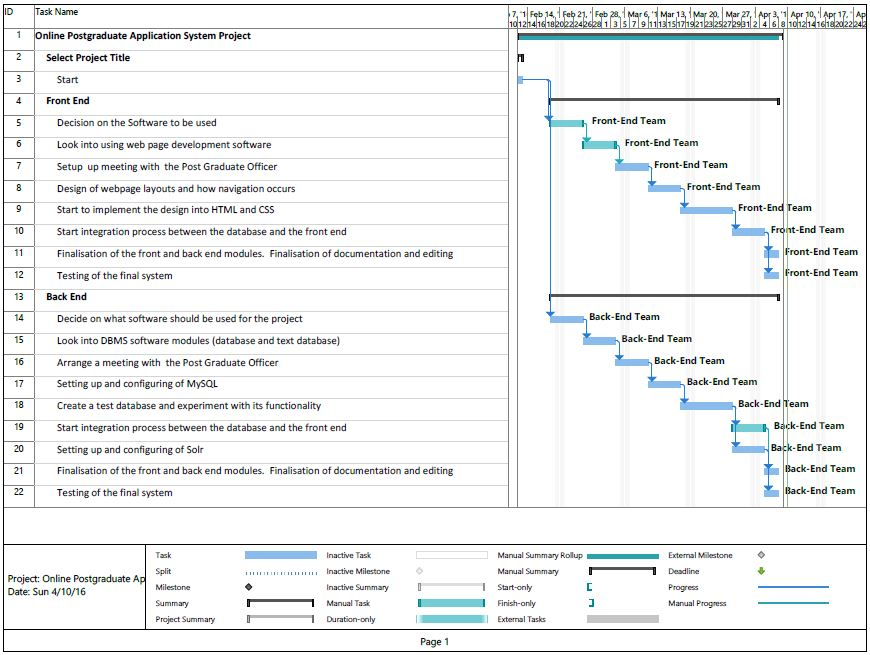
\includegraphics[width=0.7\linewidth]{GanttChart}
\caption{Gantt Chart of the work performed during the course of the Postgraduate Online Application System}
\label{GanttChart}
\end{figure}

%%%%%%%%%%%%%%%%%%%%%%%%%%%%%%%%%%%%%%%%%%%%%%%%%%%%%%%%%%%%%%%%%%%%%%%%%%%%%%%%%

\clearpage

%%%%%%%%%%%%%%%%%%%%%%%%%%%%%%%%%%%%%%%%%%%%%%%%%%%%%%%%%%%%%%%%%%%%%%%%%%%%%%%%%

\section*{Appendix B}

\begin{figure}[hbt]
\centering
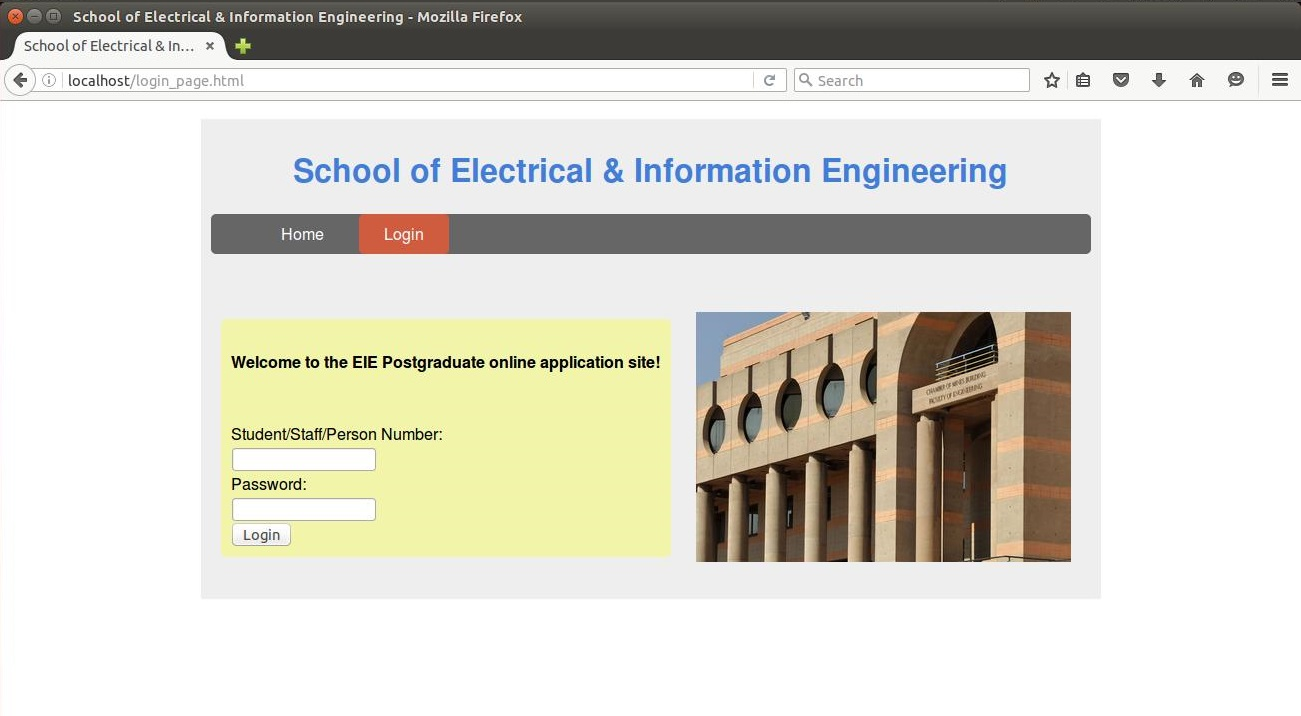
\includegraphics[width=0.7\linewidth]{loginpage}
\caption{Login page for the Postgraduate Online Application System}
\label{LoginPage}
\end{figure}

\begin{figure}[hbt]
\centering
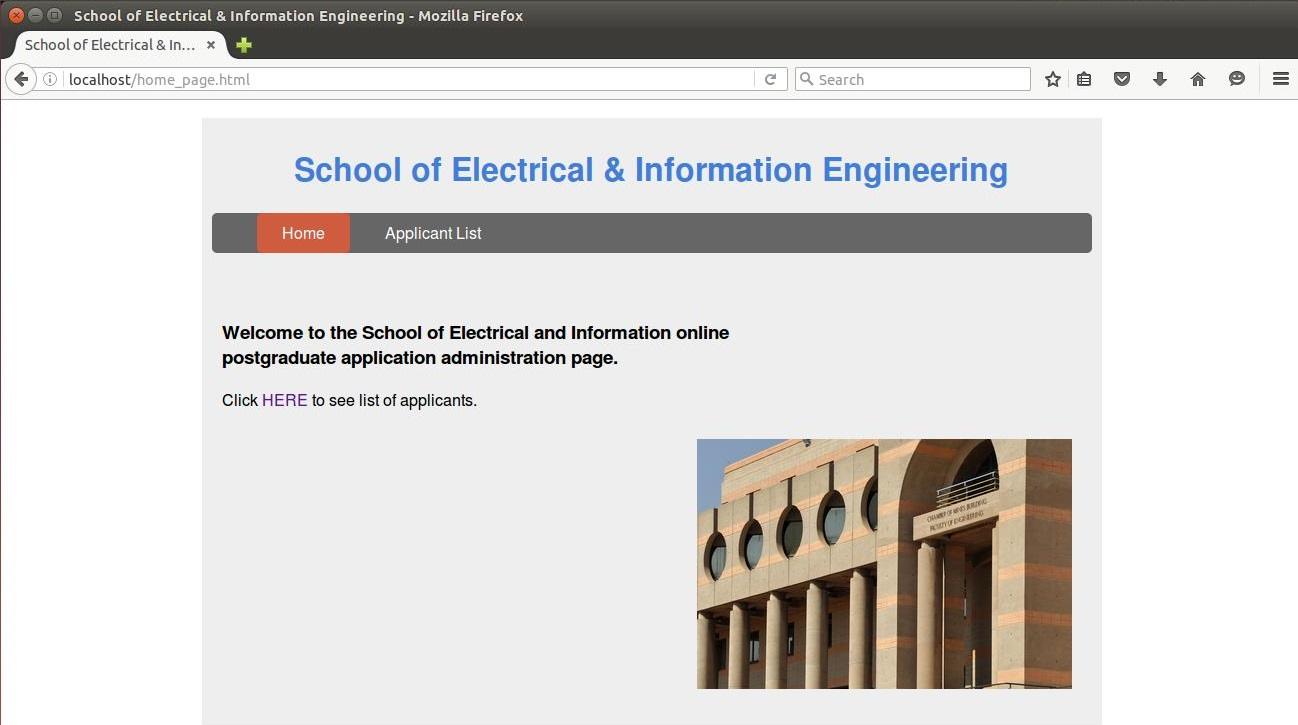
\includegraphics[width=0.7\linewidth]{home}
\caption{Home page for the Postgraduate Online Application System}
\label{HomePage}
\end{figure}

\begin{figure}[hbt]
\centering
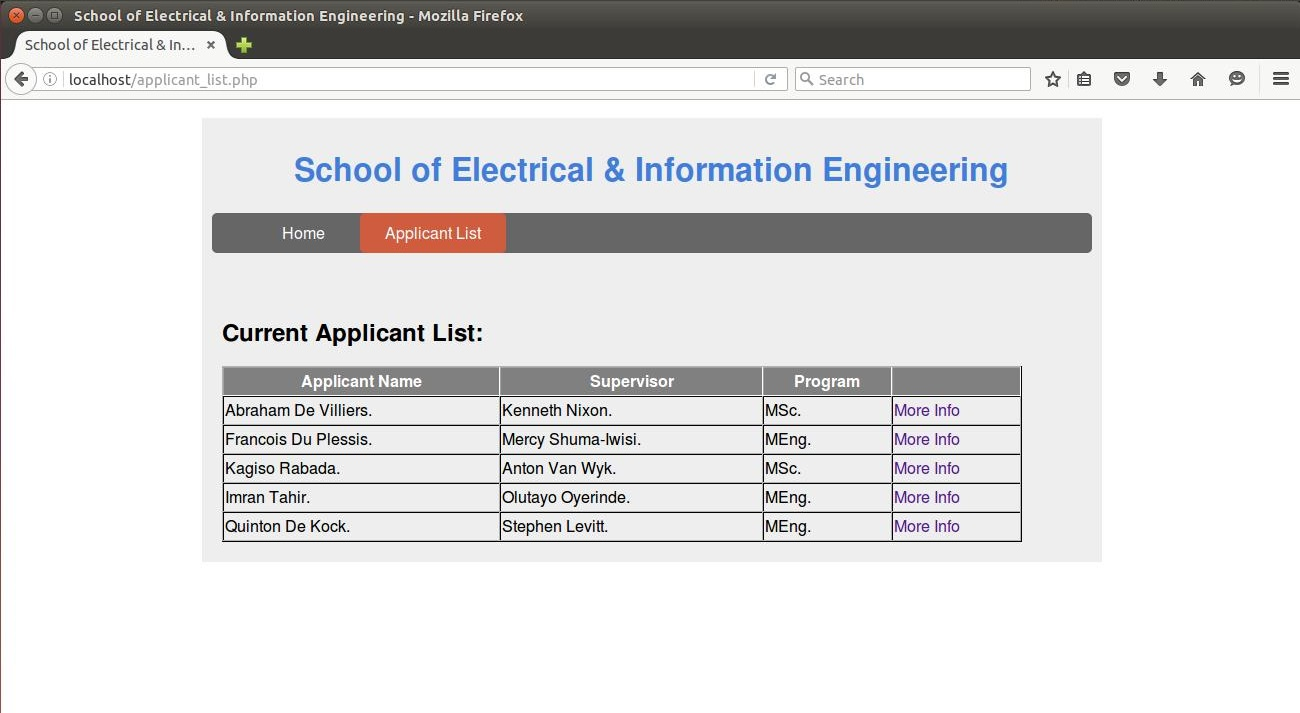
\includegraphics[width=0.7\linewidth]{list}
\caption{Applicant list page for the Postgraduate Online Application System}
\label{ApplicantList}
\end{figure}

\begin{figure}[hbt]
\centering
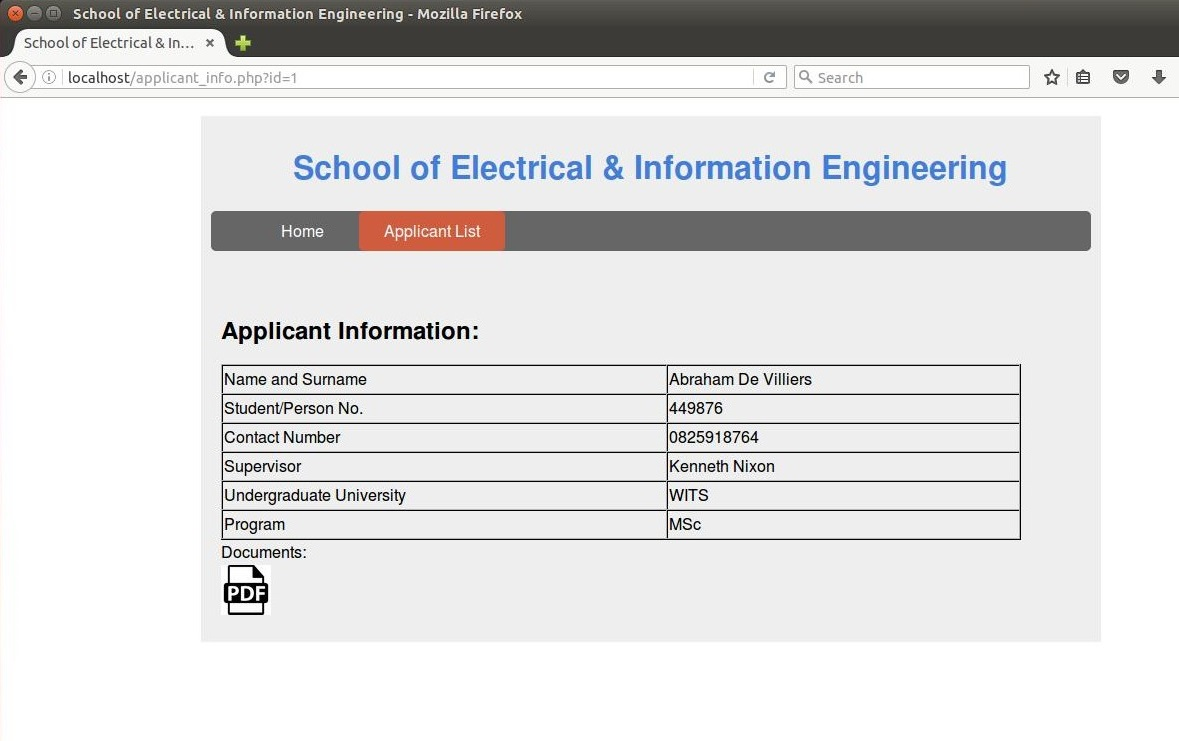
\includegraphics[width=0.7\linewidth]{information}
\caption{Applicant-specific information page for the Postgraduate Online Application System}
\label{ApplicantInformation}
\end{figure}

\begin{figure}[hbt]
\centering
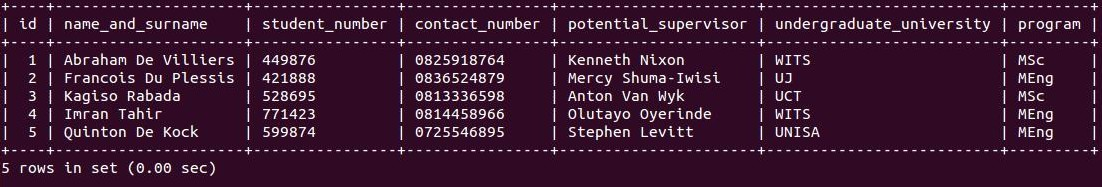
\includegraphics[width=0.7\linewidth]{mysql}
\caption{MySQL database table for the Postgraduate Online Application System}
\label{MySQLTable}
\end{figure}

%%%%%%%%%%%%%%%%%%%%%%%%%%%%%%%%%%%%%%%%%%%%%%%%%%%%%%%%%%%%%%%%%%%%%%%%%%%%%%%%%

\end{document}

%%%%%%%%%%%%%%%%%%%%%%%%%%%%%%%%%%%%%%%%%%%%%%%%%%%%%%%%%%%%%%%%%%%%%%%%%%%%%%%%%